\chapter{Introduction}

In recent years, deep learning models have demonstrated remarkable capabilities in learning from vast amounts of data, leading to broad adoption and superior performance in various real-world applications, e.g., recommender systems~\cite{Pinterest,naumovDeepLearningRecommendation2019}, content creation~\cite{openaiChatGPT2022,midjourneyMidjourney2022}, etc. As these models continue to achieve transformative results, their scale has proliferated to further enhance their competence. However, this increase in model complexity has caused a significant rise in training cost: The training cost of frontier models has grown at 2.4$\times$ annually in the last eight years. For example, training GPT-4, one of the largest models to date, incurred approximately US\$100 million. Notably, the growth in training \kwc{compute} cost has outpaced that of inference, \kwc{with the former being nearly double the latter}~\cite{villalobosTradingComputeTraining2023}.



As a result, deep learning training has increasingly posed pressing data efficiency challenges to the software computing stack. Data efficiency means effectively hiding data access latency and avoiding unnecessary data accesses. Several factors contribute to the growing importance of data efficiency. 

First, the rapid growth of large-scale models has driven an increase in GPU computational power that far outpaces improvements in data transfer bandwidth. As shown in Figure~\ref{fig:gpu_trend_various}, for recent GPUs for deep learning, FP16 throughput~(yellow dotted line, right vertical axis) has increased not only faster than memory bandwidth~(blue dotted line, left vertical axis), but also faster than the device's PCIe bandwidth~(purple dotted line, left vertical axis) and device-to-device interconnect bandwidth~(orange dotted line, left vertical axis). Moreover, hardware-accelerated lower-precision computation has enlarged the gap between the computational throughput and memory bandwidth: FP16 multiply costs 70\% less energy compared with FP32 multiply~\cite{billdallyDeepLearningHardware2022}. At the same time, FP16 data transfers only reduce energy usage by 50\% due to their proportionality to transfer size. Consequently, the training processes of most deep learning models are memory-bound. This is illustrated in Figure~\ref{fig:roofline}, where the characteristics of Nvidia B100 are compared with the deep learning training production workloads reported by Google TPU architects~\cite{jouppiTPUV4}. All models except the reported LLM workload are bound by memory. Even in LLM training, memory-intensive operations account for a significant portion of the overall execution time~\cite{liLLMAnalysisLatencyMemory2023,yuanLLMInferenceUnveiled2024}.


\begin{figure}[]
    \centering
    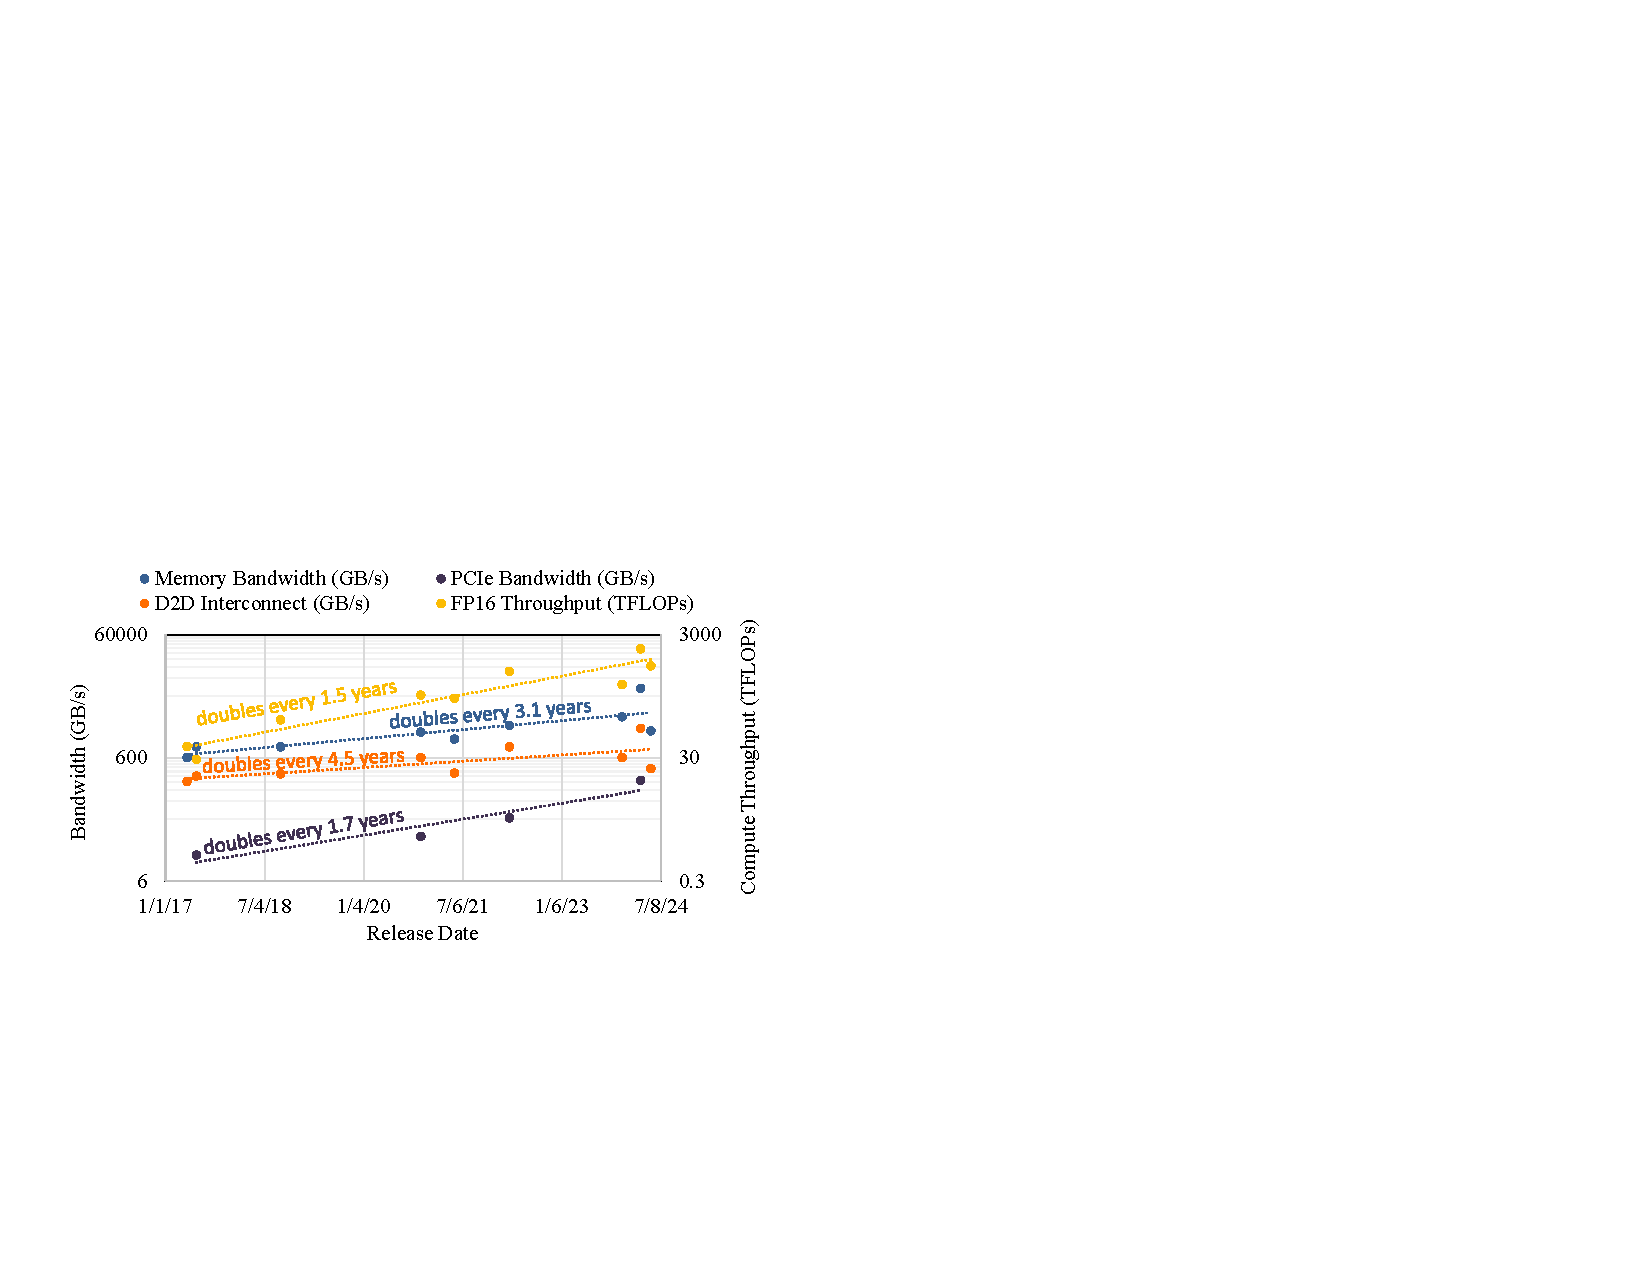
\includegraphics[width=0.8\linewidth]{figures/Intro/GPUTrendVariousHinted.pdf}
    \caption{Trend of recent GPUs for deep learning. We collect the inter-device~(D2D) bandwidth, PCIe bandwidth, memory bandwidth, and floating-point throughput of Nvidia 100-level GPUs since Kepler and Google TPUs~\cite{epochParameterComputeData,techpowerupGPUSpecsDatabase2024,jouppiTPUV4,timothyprickettmorganLotsQuestionsGoogle2024,smithNVIDIABlackwellArchitecture2024,TensorProcessingUnit2017,jouppiInDatacenterPerformanceAnalysis2017}. }
    \label{fig:gpu_trend_various}
\end{figure}


\begin{figure}[]
    \centering
    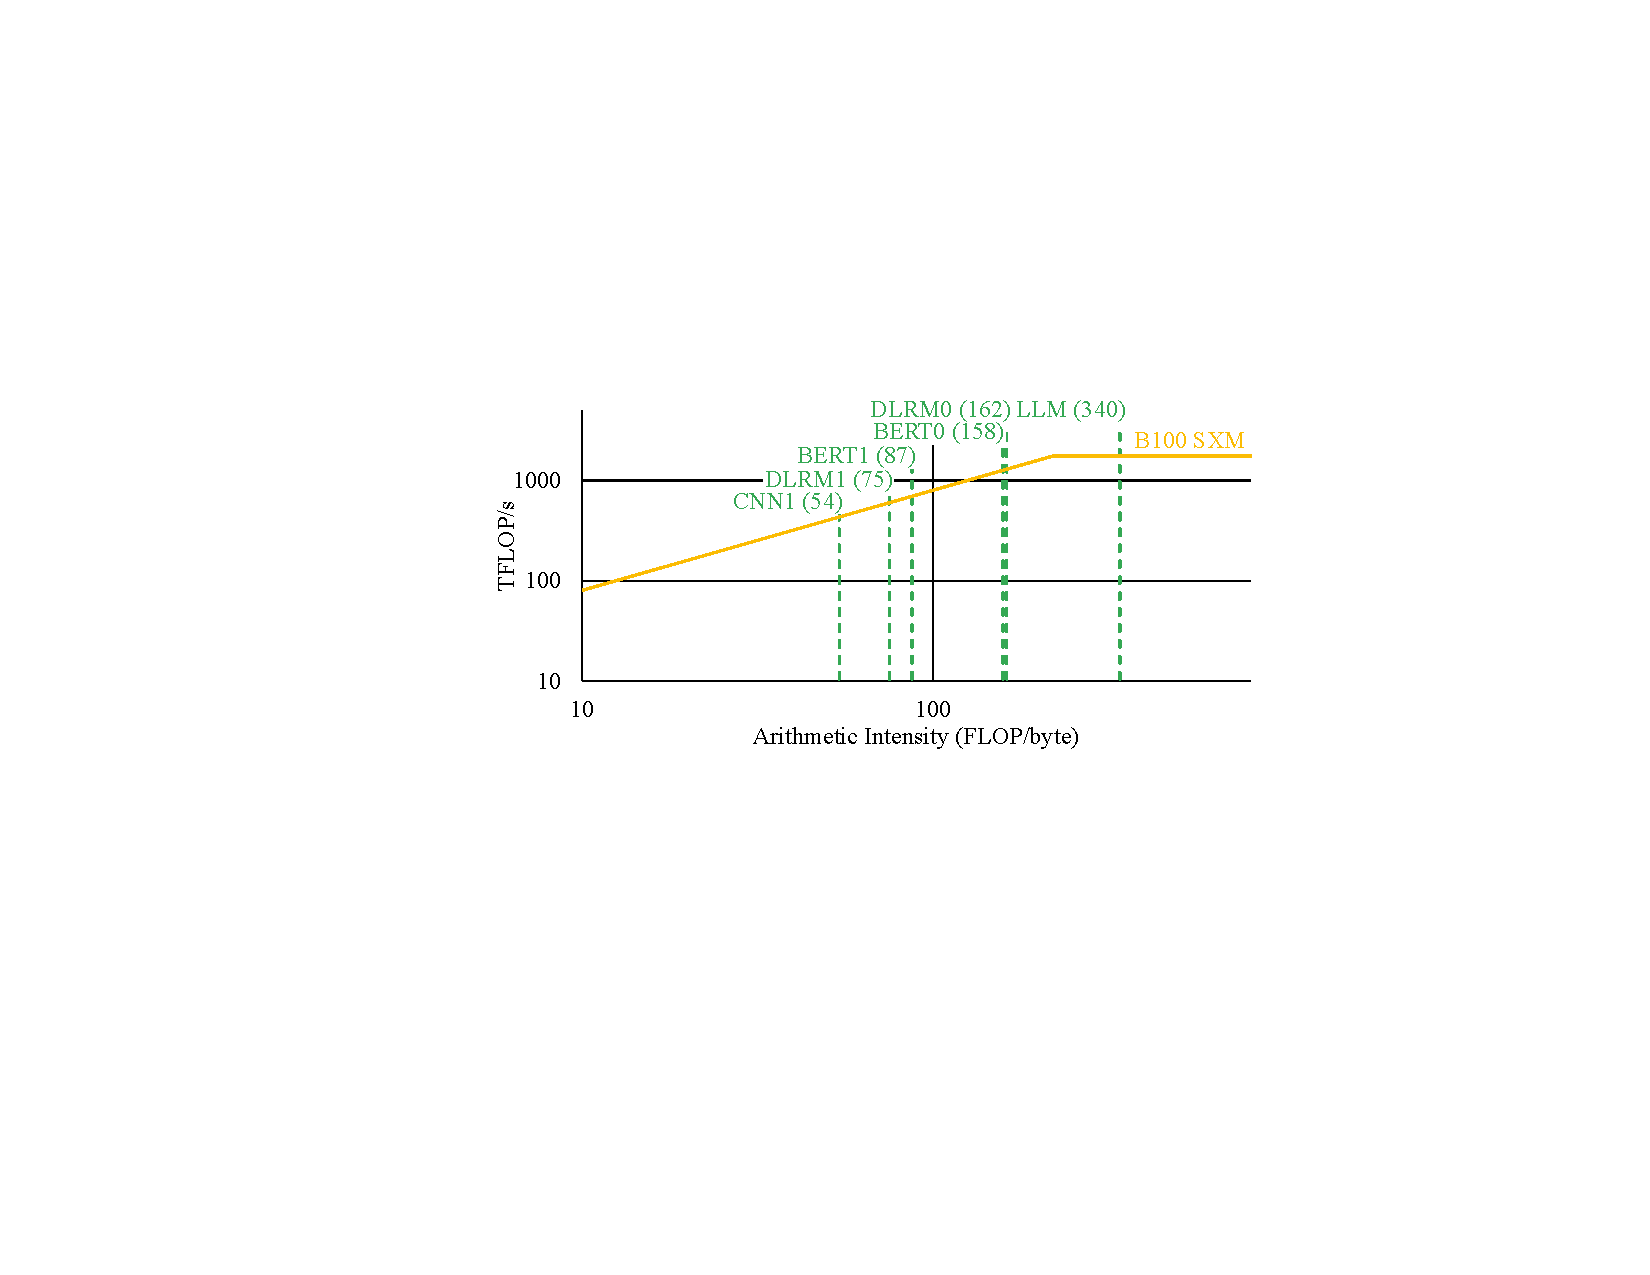
\includegraphics[width=0.8\linewidth]{figures/Intro/Roofline.pdf}
    \caption{Comparison of the memory bandwidth and FP16 throughput of Nvidia B100 SXM~\cite{smithNVIDIABlackwellArchitecture2024} with the arithmetic intensity of Google internal production workloads~\cite{jouppiTPUV4}. }
    \label{fig:roofline}
\end{figure}



Second, GPU memory capacity alone cannot sustain the growth in computational throughput, necessitating additional buffer and domain-specific PCIe transfer optimizations. Due to the limited capacity of GPU memory, deep learning training predominantly relies on mini-batches, where the entire training dataset is stored outside the GPU, and only a small subset is transferred during each step. For graph neural networks~(GNNs), the generic mini-batch transfer scheme---where the CPU prepares the mini-batch input and initiates direct memory access (DMA) PCIe transfer---introduces significant performance overhead due to fine-grained, gather-style random accesses. This can even lead to the loss of scalability~\cite{minLargeGraphConvolutional2021}. As EMOGI demonstrates~\cite{minEMOGIEfficientMemoryaccess2020,minLargeGraphConvolutional2021,minFinegrainedMemoryAccess2022}, an optimized GPU-centric transfer scheme avoids these issues by programming the GPU to use zero-copy techniques, allowing it to gather features and perform PCIe transfers simultaneously. 



For large language models~(LLMs), the growth in GPU memory capacity and main memory capacity has struggled to keep up with the increasing demands driven by GPU throughput. In contrast, SSDs offer large storage capacity, and their growth has kept up with these demands. Section~\ref{sec:llm_scaling} details the reasoning. Given this, we choose to offload tensors to SSDs for LLM training to overcome GPU memory limitations. Nevertheless, SSD bandwidth is limited, and the gap between SSD bandwidth growth and GPU computational throughput growth continues to widen, as shown in Figures~\ref{fig:gpu_trend_various} and~\ref{fig:ssd_trend_bandwidth}. It is essential to carefully manage data transfers to prevent training throughput from being constrained by SSD bandwidth. We propose techniques for selecting which tensors to offload and hiding transfer latency. To evaluate the trade-off between performance and memory savings, we compare different strategies, i.e., tensor recomputation, offloading, and keeping tensors in GPU memory. These are detailed in Chapter~\ref{ch:ssdtrain}.


\begin{figure}[]
    \centering
    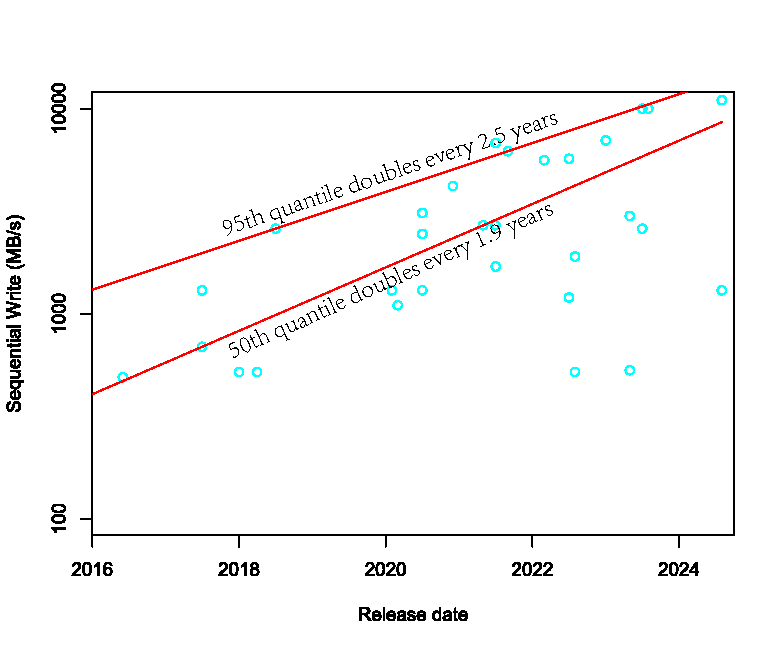
\includegraphics[width=0.8\linewidth]{figures/Intro/SSDTrendBandwidth.pdf}
    \caption{The trend of enterprise SSD sequential write bandwidth~\cite{techpowerupEnterpriseSSDDatabase2024}. For each SSD model, only the data of the variant with maximal capacity is collected. Red lines show the growth rates predicted by quantile regression. The visualization code is adapted from Derek Jones's work~\cite{derekjonesShapeCodeMemory2020}. }
    \label{fig:ssd_trend_bandwidth}
\end{figure}

\kwc{Despite the importance of data efficiency, several obstacles exist to address it within the current PyTorch-based deep learning training software stack.}
As one of the most popular deep learning frameworks, PyTorch offers an intuitive interface through the dynamic Python language. It abstracts away the complexity of CUDA-accelerated systems, making them user-friendly and fostering a robust ecosystem in the deep learning community. However, PyTorch is by no means a ``silver bullet''~\cite{brooksNoSilverBullet1987}. Instead, the PyTorch stack design is largely compute-oriented. This focus creates significant challenges when attempting to tackle data efficiency, a new paradigm requiring optimizing data access alongside computation.



\kwc{One significant challenge posed by PyTorch's compute-centric design, which we encountered while integrating the EMOGI PCIe transfer scheme}~\cite{minEMOGIEfficientMemoryaccess2020,minLargeGraphConvolutional2021,minFinegrainedMemoryAccess2022} \kwc{for GNNs, is its assumption that both the input and output of each operator reside on the same device to which the operator is dispatched.} However, the optimized transfer scheme uses the GPU to gather node features and perform PCIe transfer simultaneously as an integral process, demanding the input to be in the host memory.
To adopt such a data-efficient scheme and retain the PyTorch programming interface, the PyTorch runtime code has to be recompiled with the addition of a full-fledged new tensor type, its special host memory allocator, and its set of new dispatch rules. 
Chapter~\ref{ch:pytorch_direct} details our solution for incorporating EMOGI PCIe transfer into PyTorch.


Second, although PyTorch incorporates high-performance math libraries and uses them for corresponding operators~\cite{CuBLAS,CUTLASS2022}, it lacks high-level abstraction to capture domain-specific semantics. This limitation makes it difficult to safely optimize the code to eliminate redundant data movement and achieve more efficient execution schedules. For example, in relational GNNs~(RGNNs), a common operation is producing a per-edge vector, edge message, by multiplying the source node features with a weight matrix specific to the edge type. Since edges with the same edge type and source node will get the same edge message as the result, repetitive computation and output footprint can be eliminated. However, existing frameworks with generic GNN abstraction cannot leverage these optimization opportunities because they lack the necessary abstraction to capture and track edge-type-specific information. Chapter~\ref{ch:hector} details how a code generator with domain-specific intermediate representation~(IR) enables the optimization discussed above, compact materialization.



\kwc{In this thesis, we show that c}ode generation and runtime techniques can systematically mitigate the data \kwc{management} bottlenecks in deep learning training, which stem from the data-intensive nature of workloads and the oversimplification inherent in the deep learning training software stack.

To prove the dissertation statement, the dissertation examines the data inefficiency in representative scenarios in GNNs and LLMs, proposes runtime and code generation techniques to mitigate such inefficiency, and implements transparent incorporation into the PyTorch stack with good programmability and interoperability. 
The contributions of this dissertation are as follows:



\begin{itemize}
\item Hector IR and code generator for end-to-end RGNN training and inference~\cite{wuHectorEfficientProgramming2024}. RGNN execution faces significant performance challenges due to inherent memory intensiveness, the gap between the programming interface and the kernel APIs, and the high kernel optimization cost due to kernel coupling with layout and heterogeneity. To systematically address these issues, we present Hector. \kwc{Hector generates optimized CUDA kernels to eliminate redundant data movement within GPU and reduces GPU memory footprint.} The IR design decouples the model semantics, data layout, and operator-specific schedule and expresses these opportunities to integrate them into the design space. Based on a general matrix multiply~(GEMM) template and a traversal template, Hector already achieves up to 43.7$\times$ speed-up in training and inference compared to state-of-the-art systems. Linear operator reordering and compact tensor materialization obtain up to 3.8$\times$ speed-up compared to the Hector unoptimized code. Chapter~\ref{ch:hector} details Hector.
\item PyTorch-Direct, a GPU-centric data access paradigm for GNN training~\cite{min2021pytorchdirect,minLargeGraphConvolutional2021,minGraphNeuralNetwork2022}. Training GNNs on large graphs that do not fit in GPU memory suffers from significant throughput and CPU utilization overhead. By enabling GPUs to efficiently access complicated data structures in host memory directly without CPU intervention, PyTorch-Direct significantly reduces CPU utilization in GNN training, resulting in higher end-to-end training performance. For the input datasets and GNN architectures evaluated, PyTorch-Direct decreases the overall training time by up to 38.2\%. One of its key advantages is the minimal required programmer effort: Users can take full advantage of the benefits that PyTorch-Direct provides by modifying at most two lines of their original code. Chapter~\ref{ch:pytorch_direct} details PyTorch-Direct.
\item SSDTrain activations\footnote{In deep learning, activations are the tensors produced in forward propagation to be used for gradient computation in the backward propagation.} offloading framework for LLM training~\cite{wuTBAFasterLarge2024}. \kwc{After mitigating the data inefficiency in CUDA kernels and PCIe transfers, we take the next step to address higher-level data inefficiency, particularly challenges in overlapping kernels and transfers. Notice that} LLM training systems are increasingly constrained by GPU memory, with activations being one of the primary culprits. We propose SSDTrain to address this by offloading activations to Non-Volatile Memory Express (NVMe) SSDs. We demonstrate its viability in large-scale systems by modeling. We incorporate into SSDTrain a direct GPU–SSD data path and good interoperability. To fully overlap computation with data transfer, SSDTrain features asynchronous data transfer, tensor deduplication, forwarding, and adaptive offloading. The evaluation shows SSDTrain reduces the activations peak memory use by up to 47\% with negligible overhead. We introduce the recompute-offload-keep (ROK) curve to show runs with SSDTrain's offloading are on the efficient frontier in the design space. \kwc{We further analyze how the reduced activation memory use may lead to increased throughput by increasing micro-batch size and reducing pipeline parallelism bubbles.} Chapter~\ref{ch:ssdtrain} details SSDTrain.
\end{itemize}



The remaining chapters serve the following purposes:

\begin{itemize}
    \item Chapter~\ref{ch:background} introduces the background of this dissertation, involving GNNs, LLMs, the Nvidia GPU architecture and programming model, and the PyTorch computing stack.
    \item Chapter~\ref{ch:future_work} \kwc{presents a final discussion on PyTorch-Direct, Hector, and SSDTrain. Then, it explains the future work on top of this dissertation.}
    \item Chapter~\ref{ch:conclusion} concludes this dissertation.
\end{itemize}
